\selectlanguage{german}

\section{Lastenheft}
\begin{itemize}
    \item Sicherheitsaspekt
    \item Funktional 
    \item Interaktionsschnitstelle
\end{itemize}

\subsection{Muss - Anforderungen}

\subsubsection{Docker}
Docker ist ein Tool, das Anwendungen in kompakten, tragbaren Containern organisiert und ausführt. Diese Container sind von der Umgebung isoliert, in der sie laufen, was bedeutet, dass sie konsistent funktionieren, unabhängig davon, wo sie eingesetzt werden. Für dieses "Selfhosted" Projekt auf einem Raspberry Pi bietet Docker die Möglichkeit, verschiedene Dienste und Anwendungen ohne Konflikte nebeneinander auszuführen.

Durch die Nutzung von Docker kann man sicherstellen, dass jede Anwendung und jeder Service seine eigene Umgebung hat, was die Sicherheit verbessert und es einfacher macht, Updates und Änderungen durchzuführen, ohne andere Teile des Systems zu beeinträchtigen. Docker ist besonders wertvoll, wenn man mehrere unterschiedliche Anwendungen auf einem einzigen Raspberry Pi hosten möchte, da es die Verwaltung deutlich vereinfacht.\cite{Docker}

\subsubsection{Ubuntu 22.04 (LTS)}
Ubuntu 22.04 LTS, ist einer der beliebten Linux-Betriebssystemen. Sie bietet langfristige Unterstützung bis April 2027, was sie zu einer zuverlässigen Wahl für das Patient Monitoring System Projekt macht. Diese Version ist benutzerfreundlich und ideal für eine Vielzahl von Anwendungen, von Lernen und Experimentieren bis hin zu ernsthaften technischen Projekten. \cite{ubuntu}

\subsubsection{Dynamisches DNS-Management (ddclient)}
Der ddclient ist ein Tool, das speziell für die Aktualisierung dynamischer DNS-Einträge entwickelt wurde. Es ermöglicht es Geräten wie dem Raspberry Pi, die oft keine feste IP-Adresse haben, dennoch unter einem konstanten Domainnamen erreichbar zu sein. Durch die automatische Überwachung und Aktualisierung der sich ändernden öffentlichen IP-Adresse des Raspberry Pi sorgt ddclient dafür, dass der Pi auch nach einem IP-Wechsel durch den Internetdienstanbieter zugänglich bleibt. Diese Funktion ist besonders wertvoll für die Verwendung des Raspberry Pi als Home-Server für Anwendungen wie Webhosting, Dateifreigaben oder Überwachungsdienste. Die Installation und Konfiguration von ddclient ist unkompliziert und erfolgt über die Kommandozeile. \cite{ddclient}

\subsubsection{Fail2ban}
Fail2Ban ist ein entscheidendes Werkzeug zur Absicherung, die dazu dient, einen Server vor unautorisierten Zugriffsversuchen und Brute-Force-Angriffen zu schützen. Durch die Überwachung von Logdateien erkennt Fail2Ban auffällige Anmeldeversuche und blockiert die zugehörigen IP-Adressen automatisch für eine vordefinierte Zeitdauer. Mit Fail2Ban kann beispielsweise die IP-Adresse eines Geräts, das wiederholt versucht, ohne die korrekten Anmeldedaten eine Verbindung zum Server herzustellen, blockiert werden. Es lässt sich so konfigurieren, dass jede IP-Adresse, die mehr als dreimal pro Tag versucht, sich zu verbinden, gesperrt wird. \cite{Fail2ban} Diese Funktion ist besonders wichtig für die Minimierung von potenziellen Sicherheitsrisiken. Im Rahmen unseres Projekts auf dem Raspberry Pi wird Fail2Ban eine kritische Rolle spielen, indem es dazu beiträgt, die Zugriffskontrolle auf unsere Dienste wie SSH verstärken.

\subsubsection{MQTT / MQTT-Client}
Unser System wird aus mehreren verschiedenen Komponenten bestehen, die miteinander kommunizieren müssen. Diese Kommunikation muss über einen Message - Broker und das Protokoll ''MQTT'' erfolgen \cite{MQTT} . Um das Protokoll nutzen zu können benötigt es einen MQTT - Message Broker und Clients die ihre Nachrichten an diesen schicken, dass sie an die Clients verteilt werden, die darum gebeten haben Nachrichten eines Topics zu erhalten. 

\subsubsection{SMTP-Server / SMTP-Client}
Zu Zwecken der Protokollierung und Dokumentation muss das System zusätzlich zu einem Alarm eine Mail an einen eigenen Mailserver gesendet werden. Dieser Mailserver soll über das SMTP - Protokoll Mails empfangen können. Es muss somit ein Mailcow - Server eingerichtet werden  \cite{Mailcow} . Dafür müssen auch DNS - Records angepasst werden. 

\subsubsection{Raspberry und Raspberry Pi} \label{sec:raspi}
Für das Projekt soll der Raspberry Pi gewählt werden, da dieser eine einfache Anbindung mit einer Kamera erlaubt \cite{Raspberry}  \cite{Raspberry_camera}. Der Raspberry Pi erlaubt es Microcontroller und Kamera in einem kompakten Gehäuse unterzubringen.  Es soll zwei Raspberry Pis geben, die eine Detektion  durchführen (siehe Abb. \ref{fig:patient_monitoring}). Ein Raspberry Pi mit Raspberry Pi Kamera übernimmt die Bed Detektion und ein Raspberry Pi mit Kamera übernimmt die Fall Detektion. Ein dritter Raspberry Pi soll  dafür verwendet werden,  einen Alarm zu schalten. 

\begin{figure}[H]
	\hspace{-0.5cm}
	\begin{tikzpicture}
		
	
		\draw [-, dashed, gray] (4,1)-- (-4,1)--(-4,3.5) --(4,3.5) --(4,1);
		
			\node at (-2.8 ,3) {BED VIEW};
					
		\node[inner sep=0pt] (whitehead) at (2,2.5)
		{
\includegraphics[width=.05\textwidth]{images/camera.png}};
		
		\node[above] at (2.2,2.6) {\scriptsize Raspberry Pi und Kamera};
		
		\node[inner sep=0pt] (whitehead) at (0,2)
		{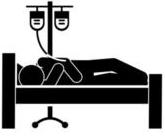
\includegraphics[width=.1\textwidth]{images/person_in_bed.png}};

			\node at (-2.6 ,-1) {ROOM VIEW};
	
			\draw [-, dashed, gray] (4,-0.5)-- (-4,-0.5)--(-4,-4) --(4, -4 ) --(4,-0.5);
		
		\node[inner sep=0pt] (whitehead) at (2,-1.5)
		{
\includegraphics[width=.05\textwidth]{images/camera.png}};
		

		
		\node[inner sep=0pt] (whitehead) at (-0.25,-1.25)
		{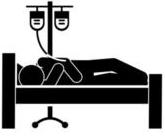
\includegraphics[width=.1\textwidth]{images/person_in_bed.png}};
		
		
		\node[inner sep=0pt] (whitehead) at (0,-2.25)
		{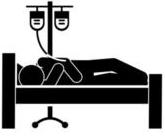
\includegraphics[width=.1\textwidth]{images/person_in_bed.png}};
		
	\node[inner sep=0pt] (whitehead) at (-0.5,-3.25)
		{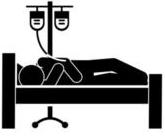
\includegraphics[width=.1\textwidth]{images/person_in_bed.png}};
		

	  \node[inner sep=0pt] (whitehead) at (4.0,0.25)
		{
\includegraphics[width=.08\textwidth]{images/server.png}};
		
				\node[below] at (2.2,-1.6) {\scriptsize Raspberry Pi und Kamera};
		
		\node[below] at (4.0,-0.1) {\scriptsize MQTT Broker};
		
			
		
		\draw [-] (2,2.5)-- ( 3,2.5) -- (3,0.25) ;
		\draw [-] (2,-1.5)-- ( 3,-1.5) -- (3,0.25) ;
		\draw [-]  (3,0.25)  -- (3.8,0.25);

	    \draw [->]  (4.2 ,0.25) -- (5.0,0.25) -- (5.0,-1.5) -- (5.5,-1.5);
	     \draw [->]  (4.2 ,0.25) -- (5.0,0.25) -- (5.0,2.5) -- (5.5,2.5);
	
		\node at  (7.0,2.5) {Bed Detection};
		
		
		\node at  (7.0,-1.5) {Fall Detection};
		
		
	
	 	\draw [->]  (8.5 ,-1.5) -- (9.0,-1.5) -- (9,0.25) -- (9.5,0.25)  ;
	
		\draw [->]  (8.5, 2.5) -- (9.0,2.5) -- (9,0.25) -- (9.5,0.25) ;
		
		\node[inner sep=0pt] (whitehead) at (9.85,0.25)
		{
\includegraphics[width=.05\textwidth]{images/raspi.png}};
		
		\node[below] at (10.,0.1) {\scriptsize Raspberry Pi };
		
		\draw [->]  (10.3,0.25) -- (10.6,0.25) ;
		
		\node[red] at  (11.2,0.25) {Alarm};
		
		
	\end{tikzpicture}
	\caption{Darstellung des Systemaufbaus}
	\label{fig:patient_monitoring}
\end{figure}


\subsubsection{Fall Detektion}
In Abschnitt  \ref{sec:raspi} wurde bereits angerissen, dass ein Raspberry Pi mithilfe der Raspberry Pi Kamera eine Fall Detektion durchführen soll. Der Raspberry Pi soll also überprüfen, ob ein Patient hingefallen ist. Dies soll mithilfe des Yolo-Frameworks gemacht werden \cite{Yolo}. Es ist hierbei Ziel das Modell auf dem Raspberry Pi zum Laufen zu bekommen, um möglichst nicht noch einen zusätzlichen Server zu benötigen. 

\subsubsection{Matrix}
Es soll einen Matrixserver geben \cite{Matrix} . Über diesen Server sollen Pfleger auch auf dem Handy benachrichtigt werden, wenn eine Alarmsituation eingetreten ist. 



\subsection{Soll - Anforderungen}

\subsubsection{Bett Detektion}
Es soll eine Komponente in unserem System geben, welche sich darum kümmert, zu erkennen, ob eine Person in einem Bett liegt. Es soll aber nicht jede Abwesenheit sofort zu einem Alarm führen, sondern nur, wenn über einen Zeitraum von 10 Minuten, das Bett leer bleibt, sollte ein Pfleger benachrichtigt werden, der dann nach dem Patienten schaut. Aufgrund der Zeitspanne von 10 Minuten, die das Bett leer bleiben muss, um einen Alarm auszulösen, ist es auch in Ordnung, wenn die Detektion etwas länger dauert. Es soll angestrebt werden, innerhalb von 30 Sekunden nach Verlassen des Betts zu erkennen das dieses leer ist. 

\subsubsection{Alarm (Ton und Licht)}
Eine wesentliche Anforderung des Projekts ist die Implementierung eines Alarmtons und eines Lichtsignals. Diese Funktionalität wird durch den Anschluss eines Lautsprechers und einer LED an den Raspberry Pi realisiert. Die Verbindung erfolgt über ein Steckbrett, auf dem auch die erforderlichen Widerstände und Transistoren montiert sind, um die Signale entsprechend zu steuern und zu verstärken.

Die LED dient dabei als visuelles Alarmzeichen, während der Lautsprecher akustische Warnungen ausgibt. Diese Komponenten werden über GPIO-Pins des Raspberry Pi gesteuert, was eine direkte Signalübertragung von der Steuerungssoftware zu den Warnsystemen ermöglicht.

\subsubsection{Firewall}
Eine Firewall ist als zusätzliche Sicherheitsebene im Projekt vorgesehen, um den Schutz des Raspberry Pi-Systems zu verstärken. Obwohl viele Heimrouter bereits mit integrierten Firewalls ausgestattet sind, ist die Implementierung einer dedizierten Firewall auf dem Raspberry Pi selbst eine wichtige Soll-Anforderung. Diese Maßnahme dient dazu, die Netzwerksicherheit weiter zu erhöhen und Anwendungsspezifische Sicherheitsrichtlinien durchzusetzen.

Die Firewall auf dem Raspberry Pi wird konfiguriert, um eingehende und ausgehende Verbindungen genau zu überwachen und zu kontrollieren. Sie filtert den Datenverkehr basierend auf vordefinierten Sicherheitsregeln und hilft dabei, unerwünschten Zugriff sowie mögliche Bedrohungen abzuwehren. Diese Schutzschicht ist besonders kritisch, wenn der Raspberry Pi in einem öffentlich zugänglichen Netzwerk betrieben wird oder sensible Daten verarbeitet.


\subsection{Kann - Anforderungen}

\subsubsection{MQTT Frontend}
Es kann ein MQTT - Frontend benutzt werden, um es Entwicklern einfacher zu machen die verschiedenen Nachrichten und Kommunikationskanäle nachzuvollziehen. 

\subsubsection{Gesprochene Information über Patient in Hilfesituation}
In den Minimalanforderungen unseres Systems weiß ein Pfleger nur das ein Patient Hilfe benötigt, nicht aber, welcher der Patienten. Um diese Problematik zu lösen, kann das System anstelle des Alarmtons über eine sprechende Stimme dem Pfleger mitteilen, welcher Patient Hilfe benötigt. 

\subsubsection{Kameraview}
Falls noch Zeit ist, soll zusätzlich mithilfe des QT-Frameworks eine Kameraview  in Python entwickelt werden \cite{Python} \cite{QT} . Mit dieser Anwendung sollen  Pfleger die Patienten überwachen können. Sie können so Dinge entdecken, die durch unsere Detektoren nicht abgedeckt werden. Ein Pfleger könnte so die Extubation eines Patienten erkennen. 
